\section{Presentazione}
\label{presentazione}
Nel definire la grafica del sito si è partiti dall'interfaccia mobile, per poi fissare ulteriori regole per gli elementi il cui aspetto doveva adattarsi a finestre più grandi. Questo si vede dalla struttura del foglio di stile \textit{Style.css}: le regole iniziali sono proprie del formato mobile, se possibile applicate anche agli altri formati; seguono le regole del formato tablet, racchiuse in un'apposita media query; infine quelle per il desktop, anch'esse in una media query. I vantaggi dell'approccio mobile first sono:
\begin{itemize}
	\item molti utenti navigano da dispositivi mobili, quindi è importante curare l'esperienza di navigazione in schermi piccoli, in particolare la grafica;
	
	\item partire dal dispositivo più piccolo va incontro al principio di responsive design (design che si adatti alle dimensioni della finestra del browser): è più facile partire da una schermata piccola e poi ingrandirla, includendo mano a mano più elementi, rispetto all'approccio inverso, che rischia, nel passaggio dal grande al piccolo,  di comprimere le informazioni in spazi troppo stretti;
	
	\item una grafica che parta dal mobile si concentra da subito sugli elementi fondamentali delle pagine, poiché deve sfruttare al meglio lo spazio a disposizione: ciò è un vantaggio nel successivo design delle finestre più ampie.
\end{itemize}

Il foglio di stile per la grafica da schermo è unico per tutti i formati, in modo da ottimizzare al massimo il codice. Allo stile di stampa è stato dedicato un secondo file, poiché molti elementi visualizzati a schermo sono eliminati dal formato di stampa, e aspetti basilari, come il font o i margini, sono diversi tra stampa e display.

\subsection{Mobile}
\label{presentazione-mobile}

\begin{center}
	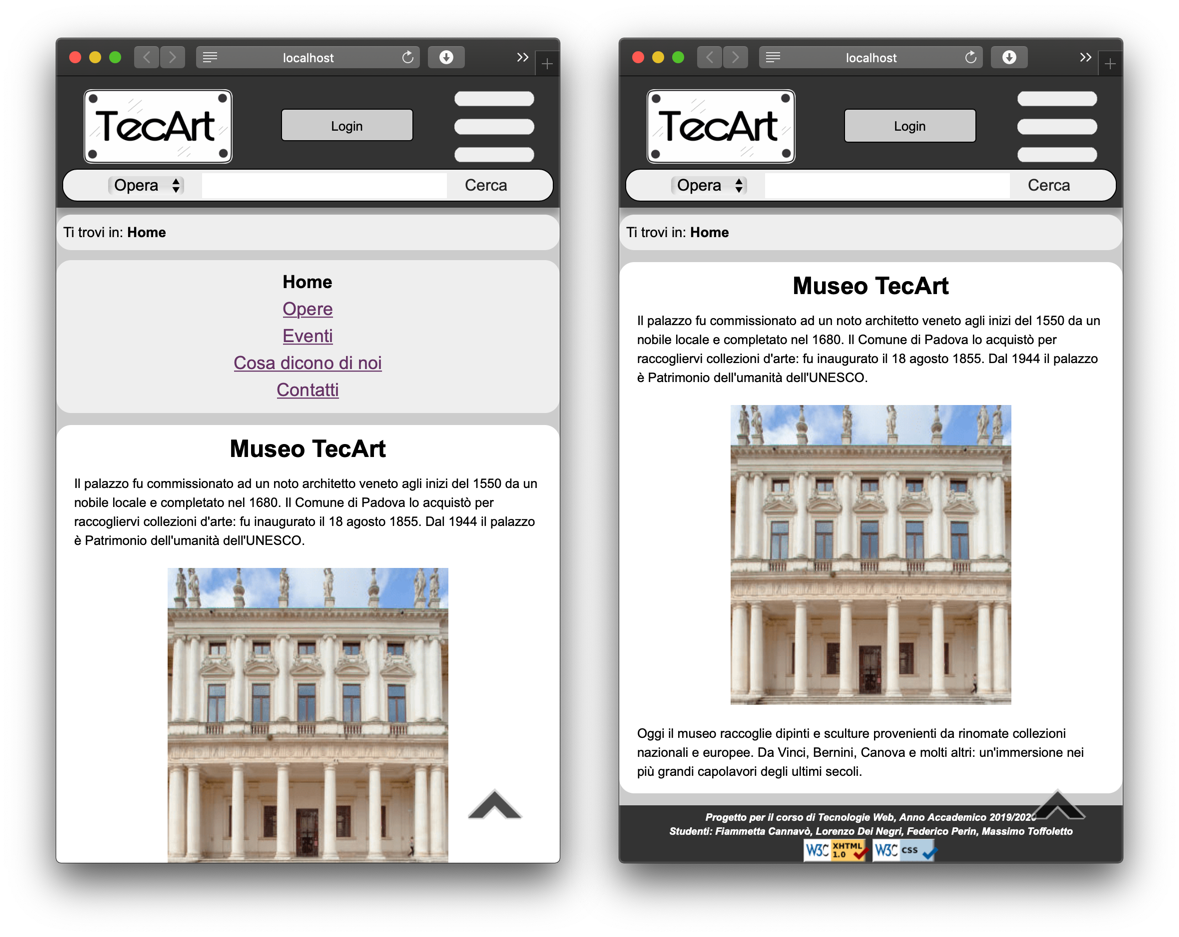
\includegraphics[scale=0.27]{img/Mobile-pres}
	\captionof{figure}{Grafica mobile con menu visibile (a sinistra) e nascosto (a destra)}
\end{center}

La grafica mobile presenta un header contenente logo, menu per il login e la gestione dell'area personale e l'icona per il menu ad hamburger. Per il menu è stata scelta un'icona, invece di un button contenente del testo, perché più coerente con la grafica adottata per le interfacce \textit{mobile}. Segue il breadcrumb e subito sotto il corpo della pagina. In fondo alla schermata si trovanp il footer e la freccia per tornare all'inzio della pagina senza scroll verticale. Cliccando sull'icona ad hamburger, sotto il breadcrumb compare il menu, altrimenti non visualizzabile. Si è deciso di nascondere il menu del sito per evitare di occupare la schermata, già piccola, con contenuti diversi dal corpo della pagina.

\subsection{Tablet}
\label{presentazione-tablet}

\begin{center}
	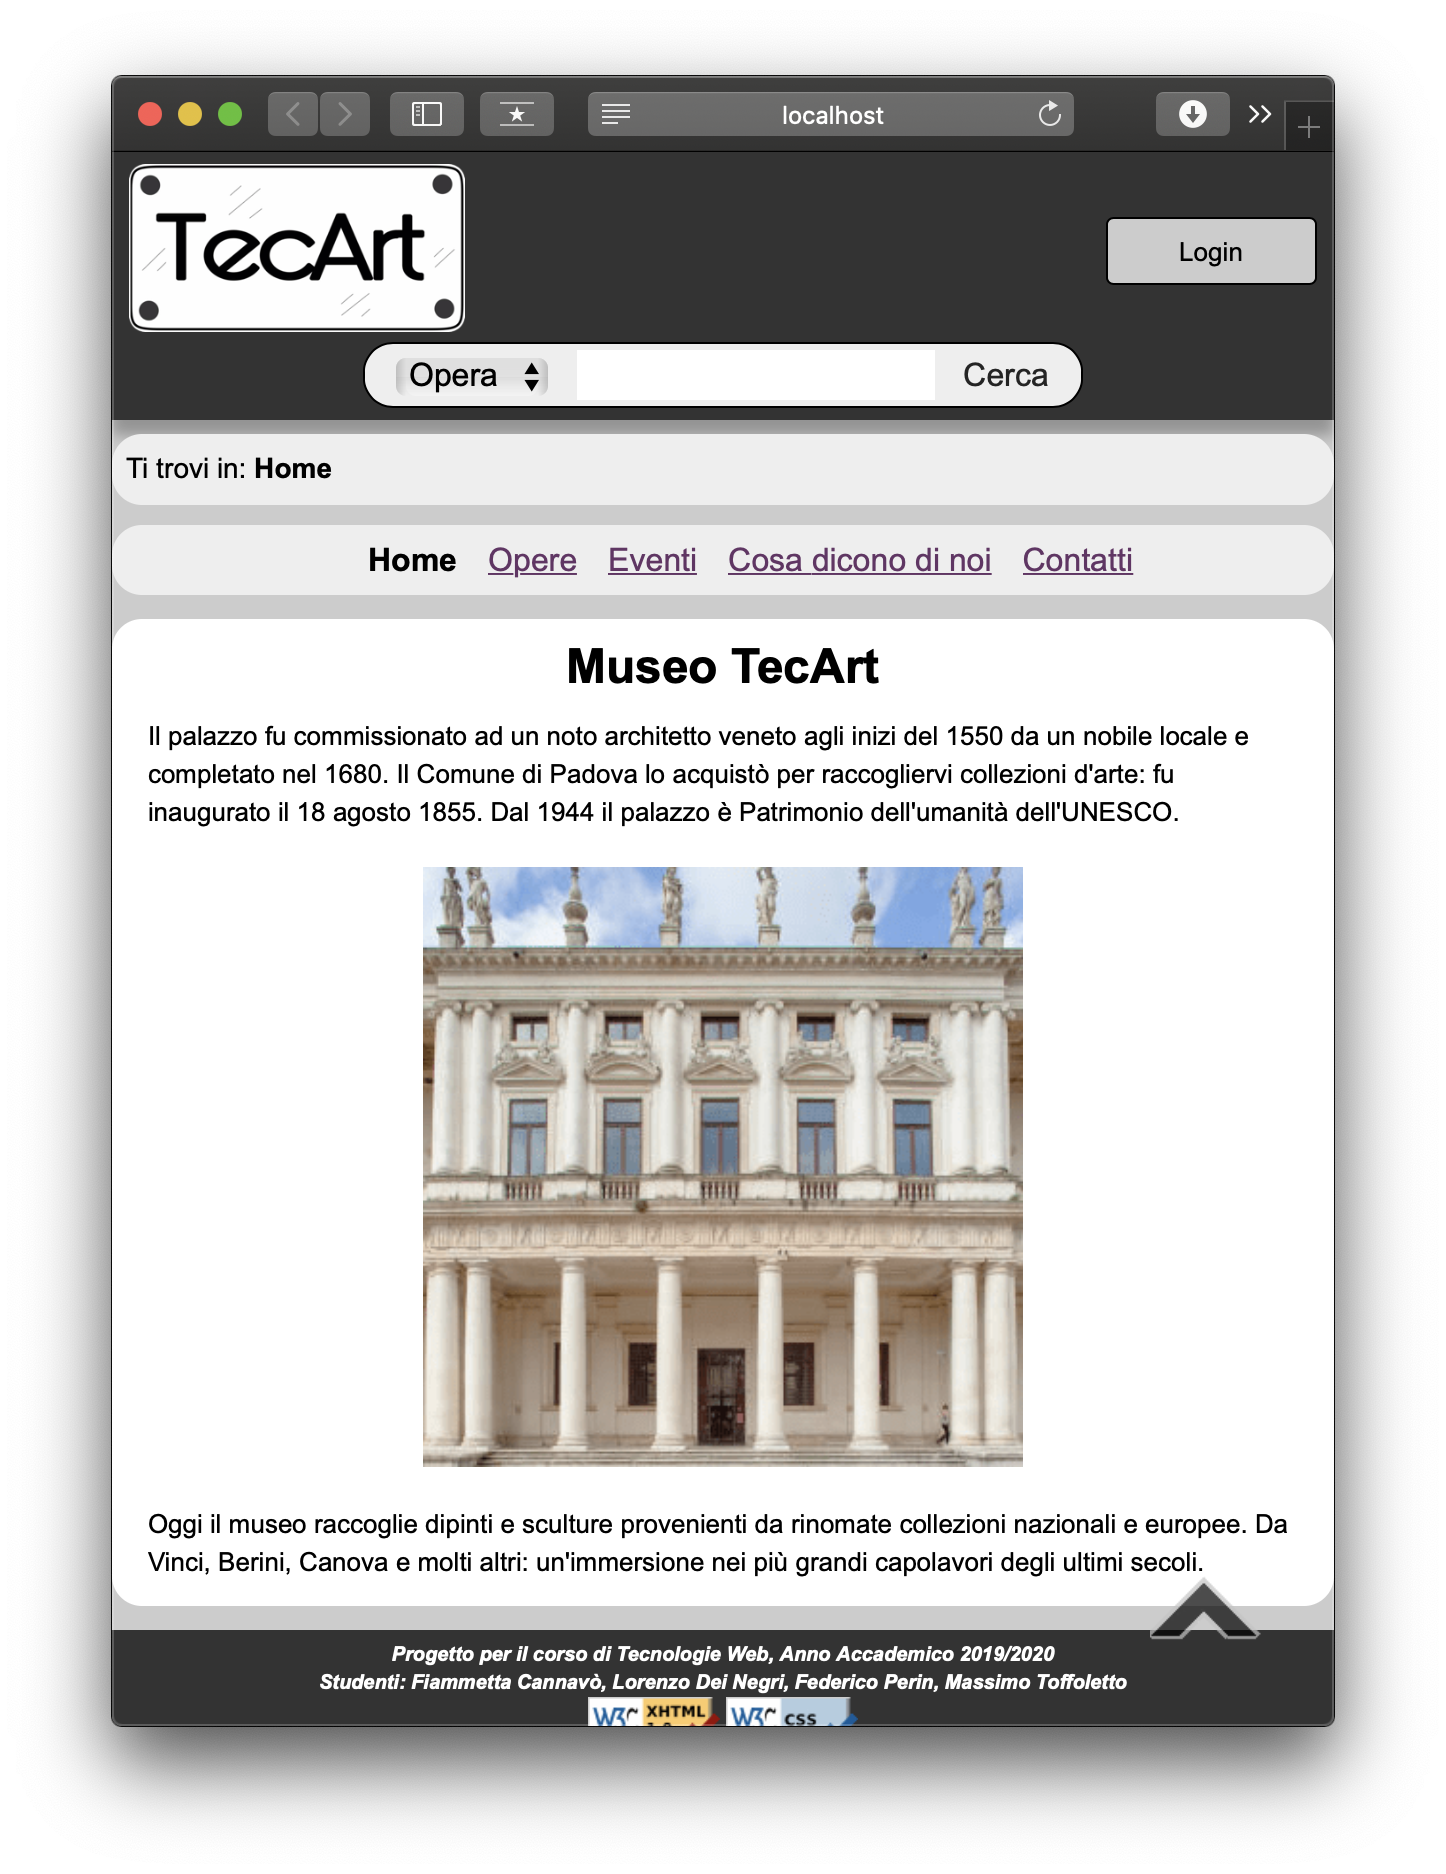
\includegraphics[scale=0.45]{img/Tablet-pres}
	\captionof{figure}{Grafica tablet}
\end{center}

La peculiarità del formato tablet è la posizione del menu: scompare l'icona ad hamburger e il menu è spostato sotto il breadcrumb. I link non sono più incolonnati ma posti in un'unica riga: in questo modo si evita di rubare troppo spazio al corpo della pagina, ma allo stesso tempo, essendo la schermata più ampia rispetto a quella di uno smartphone, si evita che l'utente debba effettuare un click per visualizzare il menu.


\subsection{Desktop}
\label{presentazione-desktop}

\begin{center}
	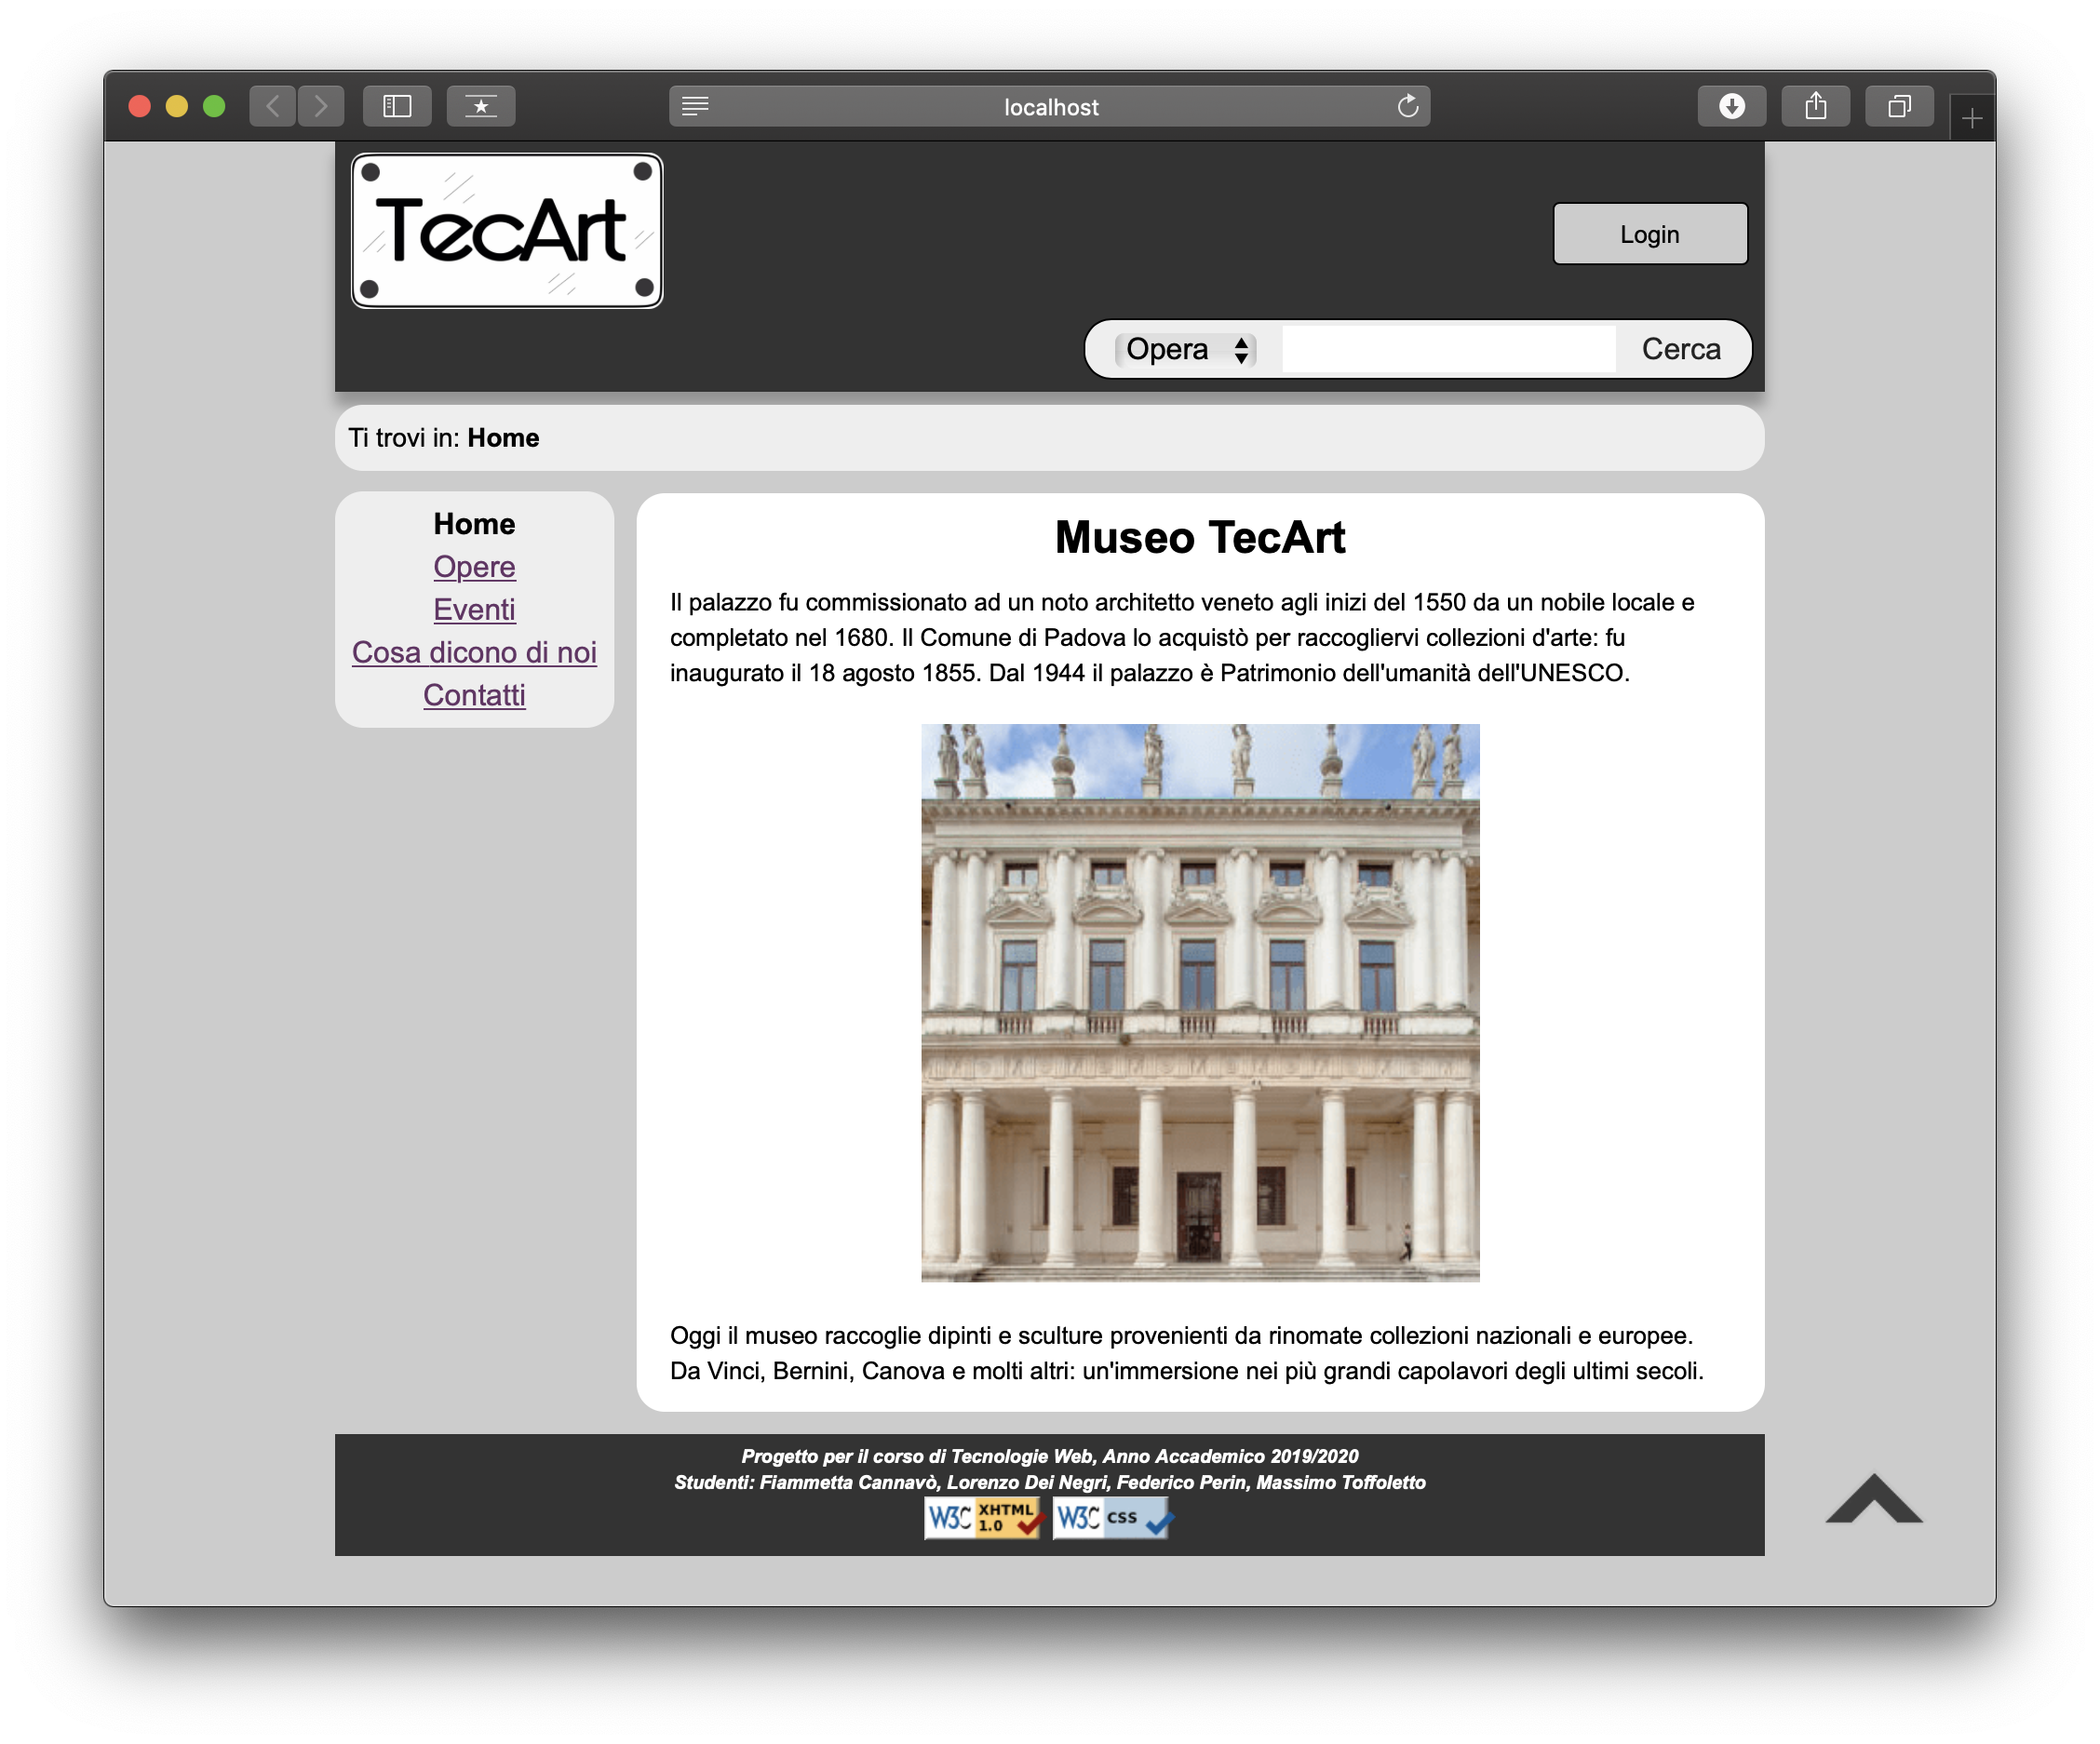
\includegraphics[width=\textwidth]{img/Desktop-pres}
	\captionof{figure}{Grafica desktop}
\end{center}
Ancora una volta, a cambiare è l'aspetto del menu: avendo a disposizione una finestra ampia è possibile mantenere il menu sempre a schermo, posizionandolo però sul lato sinistro, in modo da lasciare più spazio possibile, in verticale, al contenuto della pagina. Per garantire un'esperienza positiva di navigazione anche agli utenti con uno schermo piccolo, si è deciso di limitare l'ampiezza massima della finestra a 1024px, eventualmente occupando il resto della finestra con uno sfondo uniforme, in liena con la palette di colori del sito.


\subsection{Stampa}
\label{presentazione-stampa}

%\begin{center}
%	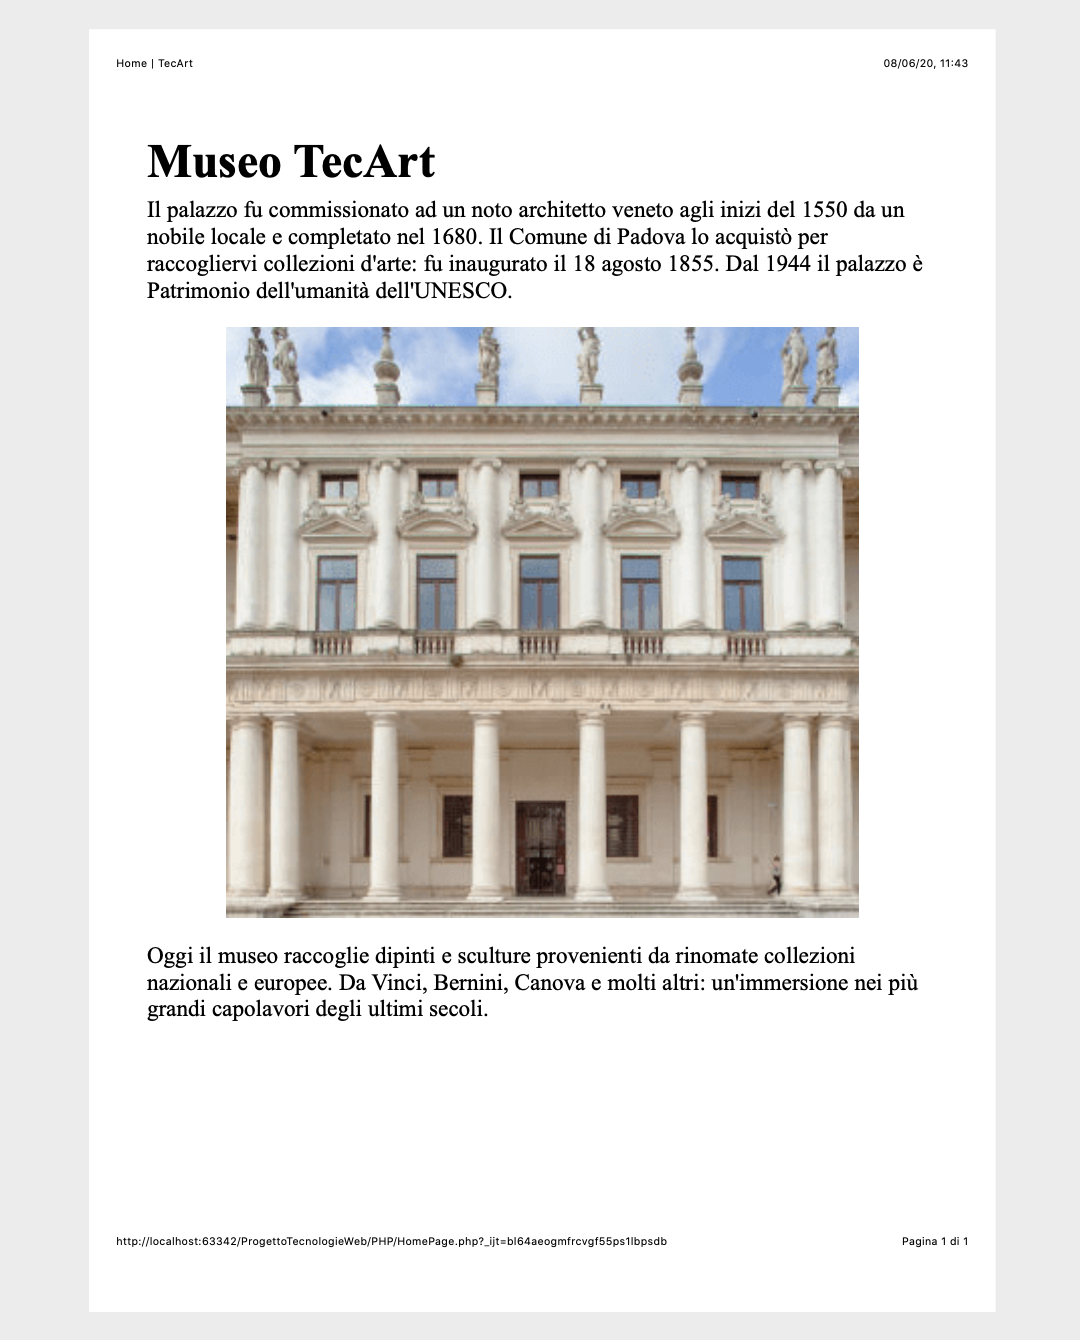
\includegraphics[scale=0.16]{img/Stampa-pres}
%	\captionof{figure}{Grafica stampa}
%\end{center}

Il layout di stampa omette tutti i sopporti alla navigazione: non compaiono i menu, il breadcrumb e i button. Sono rimosse anche tutte le immagini non significative, anche se si è ritenuto opportuno mantenere quelle delle opere, trattandosi del sito di un museo di opere d'arte.
